% Chapter Template

\chapter{Implementierung} % Main chapter title

\label{Chapter5} % Change X to a consecutive number; for referencing this chapter elsewhere, use \ref{ChapterX}

\lhead{Chapter 5. \emph{Implementierung}} % Change X to a consecutive number; this is for the header on each page - perhaps a shortened title

%----------------------------------------------------------------------------------------
%	PRAXIS
%----------------------------------------------------------------------------------------

%
% AUFBAU
%
In diesem Kapitel wird darauf eingegangen, aus welchen Komponenten der im Rahmen dieser Arbeit entwickelte IICMChecker (\textbf{I}nter-\textbf{I}nstance \textbf{C}onstraints \textbf{M}odel \textbf{C}hecker) zur Überprüfung auf Einhaltung von Einschränkungen bei Prozessen auf Log-Basis aufgebaut ist und welche Funktion sie haben. Das Programm ermöglicht die Eingabe von Einschränkungen und Regeln im Intra-Instance sowie im Inter-Instance Kontext in einer intuitiven, an die natürliche Sprache angelehnte Eingabesprache. Diese Regeln werden in einem Container abgelegt, der sie in Klauseln im Prolog Format konvertiert. Ebenfalls werden einige Optimierungen und zusätzliche Prädikate hinzugefügt, die sicher stellen, dass die Regeln im richtigen Kontext angewandt werden.

\begin{figure}[ht]
	\centering
  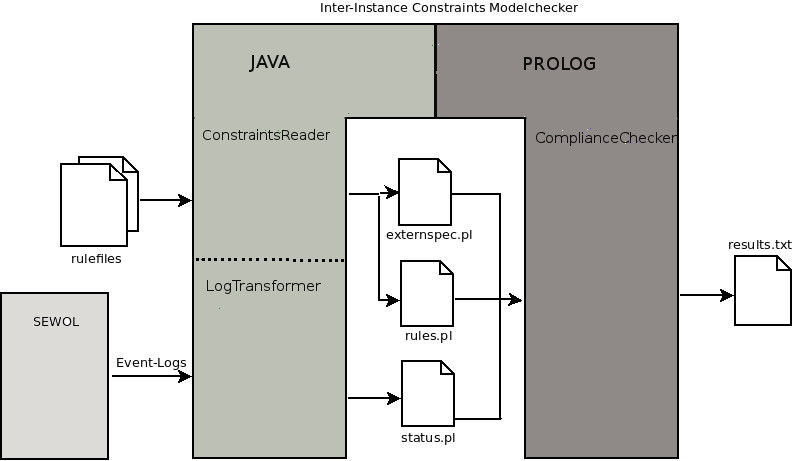
\includegraphics[width=0.9\textwidth]{Figures/Programm}
	\caption{Aufbau des IICMCheckers}
	\label{fig:myprog}
\end{figure}
Das Programm besteht aus drei Teilen die über Prologdateien miteinander kommunizieren, wobei die lesenden Teile in Java implementiert sind und der ausführende Teil (der eigentliche Modelchecker) in Prolog ausgeführt wird.
Der Logtransformer liest Logs im SEWOL \cite{SEWOL} Format ein und übersetzt sie in Status Prädikate (siehe Abschnitt \ref{sec:logtransformer}). 
Die Constraints werden ebenfalls vom Constraintreader (siehe Abschnitt \ref{sec:constraintreader}) eingelesen und in Regelprädikate übersetzt.
Der Compliancechecker selbst ist in Prolog geschrieben und liest dazu die zuvor erstellten Statusprädikate und Regeln (für näheres siehe Abschnitt \ref{sec:compliancechecker}). Im letzten Abschnitt \ref{sec:results} wird noch kurz darauf eingegangen, wie die Ergebnisse des ComplianCecheckers interpretiert werden müssen.

\section{Verwendete Hilfsmittel}
\subsection{SEWOL}
SEWOL (\textbf{SE}curity-oriented \textbf{WO}rkflow \textbf{L}ib) wird am Institut für Informatik und Gesellschaft an der Universität Freiburg entwickelt. SEWOL ist eine Bibliothek, die das Arbeiten mit Prozesslogs unterstützt. Es bietet unter anderem die Möglichkeit, Logs in einfacher Text-Form, MXML und XES Format zu parsen und auch zu serialisieren. Ein Log besteht aus mehreren \textit{traces}, wechels wiederum eine Liste von Log Einträgen enthält. Ein einzelner Eintrag repräsentiert dabei ein Event einer einzelnen Aktivität in einem Prozess. Zu jedem Logeintrag können zusätzliche Informationen hinzugefügt werden, wie der Zeitpunkt der Ausführung, der Nutzer (die Person oder das System, welcher für die Ausführung verantwortlich ist), die Rolle des Nutzers, den Typen des Events (start, complete,..) und weiteren Meta Informationen, die in Form von \textit{DataAttributes} hinzugefügt werden können. \cite{SEWOL}
\subsection{ANTLR}
ANTLR (\textbf{AN}other \textbf{T}ool for \textbf{L}anguage \textbf{R}ecognition) ist ein objektorientierter Parser Generator, der dazu geeignet ist, strukturierten Text zu lesen, zu bearbeiten, zu übersetzen und auszuführen. Die Applikation wird seit 1989 von Terence Parr an der Universität von San Francisco entwickelt und ist als freie Software verfügbar.\\
Eine vom Nutzer definierte Grammatik wird zuerst von einem Lexer verarbeitet und der entstehende Tokenstream anschließend geparst. Die Grammatik selbst ist in Parser und Lexer Regeln aufgeteilt. Zu der Grammatik erstellt ANTLR einen \textit{parse tree}, welcher eine Datenstruktur ist, die repräsentiert, wie eine Grammatik den gelesenen Text interpretiert. Zudem wird ein entsprechender \textit{parse tree walker} und \textit{listener} erzeugt, die den \textit{parse tree} durchlaufen und gemäß der Implementierung des \textit{listeners} verarbeiten.\\
ANTLR selbst in in Java geschrieben.\cite{antlr}
\subsection{Programmiersprachen} 
Die Regeldefinition erfolgt in der eigens dafür entwickelten Grammatik (Kapitel \ref{GrammatikKapitel}). Das Einlesen der Logs sowie deren Konvertierung als auch das Übersetzen der Grammatik wurde in Java implementiert. Alle Informationen werden in Prolog Klauseln und Regeln übersetzt, welche mit dem Compliancechecker in Prolog ausgewertet werden.

%
% ARCHITEKTUR UND UMSETZUNG
%
\section{Architektur und Umsetzung der Analyse}
\subsection{Erstellen der Wissensbasis - Einlesen der Logs}
\label{sec:logtransformer}
Um dem Compliancechecker die Informationen in einem verwendbaren Format als Prolog Klauseln liefern zu können, werden die Logs mittels SEWOL eingelesen. Der Logtransformer erstellt daraufhin für jeden einzelnen Eintrag je nach enthaltenen Informationen Klauseln aus sieben möglichen Prädikaten her, die in der Datei \textit{Status.pl} im Ordner \textit{prologfiles} gespeichert werden. 
Die \textbf{taskID} wird dabei automatisch generiert, um zusammengehörige Einträge zu identifizieren. Die restlichen Argumente entsprechen den Informationen, die zu den jeweiligen Aktivitäten herausgelesen werden konnten. Sollte ein Eintrag nicht vorhanden sein, wird er nicht gesetzt und gilt bei der späteren Untersuchung bei einer Anfrage \textbf{false} zurück.


\begin{table}[h!]
\begin{tabular} {|p{6cm}|p{10cm}|}
\hline
\textbf{Prädikat} & \textbf{Beschreibung}\\
\hline
\small workflow{\_}name(caseID,workflowName)& Weist einer Case ID einen eindeutigen Namen hinzu, welcher der Workflow Spezifikation entspricht. Die Case ID kennzeichnet die Instanz, konkrete Ausführung eines Workflows. Dieses Prädikat dient jedoch nur zur Vollständigkeit. Sollte es für den Arbeitsablauf keinen eindeutigen Namen geben, wird dieses Prädikat nicht gesetzt. Es kann im Modelchecker dann auch nicht darauf zugegriffen werden.\\
\hline
\small task{\_}workflow(taskID, caseID)& Setzt fest, zu welcher case ID die Activity gehört. TaskID wird intern vom Transformer gesetzt.\\
\hline
\small task{\_}name(taskID,taskName)&Legt den Namen der Activity fest. Dieser ist im MXML Modell als WorkflowModelElement zu finden. \\
\hline
\small timestamp(taskID,timestamp)&Zeitpunkt der Aktivität in ms nach 1970. \\
\hline
\small eventtype(taskID,eventtype)& Events, wie sie in Abschnitt \ref{sec:activities} - Aktivitäten vorgestellt werden. Es ist möglich, die Events neu zu definieren.\\
\hline
\small executed{\_}user(user,taskID)&Der Nutzer, der die Activity ausgeführt hat. \\
\hline
\small executed{\_}group(group,taskID)&Die Rolle, in der die Activity ausgeführt wurde. Man beachte, dass ein Nutzer mehrere Rollen haben kann.\\
\hline
\small task{\_}attribute(taskID, attrName, attrValue)& Alle weiteren Attribute, die in SEWOL unter MetaAttributes stehen. Das zweite Argument ist der Name des Attributs und das dritte Argument der Wert des Attributs. Die Werte werden entweder als String gespeichert, oder - wenn möglich - als Nummer, um später Vergleiche und arithmetische Operationen zu ermöglichen. \\

\hline
\end{tabular}
Diese Statusprädikate werden aus den Logs extrahiert und sind ausschließlich dem Modelchecker sichtbar. Sie sind nicht zu verwechseln mit den Prädikaten, die in der Grammatik verwendet werden. 
\caption{Statusprädikate}
\label{tab:statuspr}
\end{table}


\newpage
Die ersten 2 Zeilen aus Tabelle \ref{tab:examplelog} werden somit in die Wissensbasis aus Tabelle \ref{tab:knowledge} konvertiert.
\begin{table}[h!]
\begin{tabular}{ccc}
task{\_}workflow(0,0)&task{\_}workflow(1,0)\\
task{\_}name(0,'Approach check')&task{\_}name(1,'Pay check')\\
timestamp(0, 123)&timestamp(1, 123)\\
eventtype(0, start)&eventtype(1, start)\\
executed{\_}user(0, 'Mark')&executed{\_}user(1, 'Theo')\\
executed{\_}role(0, 'Admin')&executed{\_}role(1, 'Azubi')\\
task\_attribute(0, 'amount', 3000)& task\_attribute(1, 'amount', '3000Euro')\\
\end{tabular}\\\\
\small Aus einem Log herausgelesene Klauseln in Prolog. Die TaskID wird für jeden Eintrag automatisch generiert. Die restlichen Informationen stammen aus dem Log. Diejenigen Attributswerte, die eine valide Zahl darstellen, werden auch als Zahl gespeichert, um arithmetische Operationen zu erlauben. Die restlichen Werte werden als String im Prolog Format (zwei einfache Anführungszeichen) gespeichert. 
\caption{Wissensbasis}
\label{tab:knowledge}
\end{table}


%
% EINGABE DER REGELN
%
\subsection{Übersetzung der Regeln}
\label{sec:constraintreader}

Der Parser und Listener für die Grammatik wurde mit ANTLR 4.5 \cite{antlr} erzeugt. Die Grammatik selbst wird in einfachen Textdateien ohne Endung im Ordner \textit{rulefiles} abgelegt \footnote{Im Anhang B - Argumente und Konfiguration wird beschrieben, wie sich der Quellordner und Dateinamen manuell anpassen lassen.}. Während der Parse Tree Walker den Parse Tree durchläuft, fügt der Listener die gefundenen Klauseln und Regeln den entsprechenden Containern hinzu. Gleichzeitig werden weitere Klauseln gesetzt, die notwendig sind, um den entsprechenden Kontext sicherzustellen. Sobald alle Regeln gesetzt sind, lässt der \texttt{StorageHelper} alle Container die enthaltenen Informationen in geordneter Reihenfolge in Prologdateien ablegen. Aus der Grammatik entstehen zwei Dateien \textit{externspec.pl}(hier stehen alle Klauseln aus den \texttt{SET} Operationen) und \textit{rules.pl} ( die Regeln im \texttt{IF} body \texttt{THEN} head Abschnitt) im Ordner \textit{prologfiles}.\\

\textbf{Container Datenstruktur}\\
Die Container sind eine Datenstruktur, in der alle Klauseln und Regeln zuerst abgelegt werden, um sie später geordnet und geprüft als Prologklauseln in Dateien ablegen zu können. Es gibt drei Container: \texttt{ExternAndSpecificationContainer}, \texttt{StatusContainer} und der \texttt{RuleContainer}. Im \texttt{StatusContainer} liegen alle Informationen, die aus den Logs gelesen werden. \newline
Der \texttt{ExternAndSpecificationContainer} enthält alle Klauseln, die in den Rulefiles gesetzt werden. Es sind nur Prädikate aus den Tabellen \ref{tab:extern} und \ref{tab:specification} erlaubt. Zusätzlich ist es möglich, eigene Prädikate zu definieren, die ebenfalls in diesem Container abgelegt werden. Zuletzt wird der \texttt{RuleContainer} mit den eigentlichen Einschränkungen befüllt. Diese widerum können nur Prädikate aus Tabelle \ref{tab:head} im Kopf der Regel enthalten, und werden nach diesen fünf Prädikaten gegliedert (\texttt{UserCannotDoRule}, \texttt{UserMustDoRule}, \texttt{RoleCannotDoRule}, \texttt{RoleMustDoRule} und \newline
\texttt{IllegalExecutionRule}), die alle die abstrakte Klasse \texttt{Rule} erweitern. Jede Regel enthält einen \texttt{Rule\_Body} in welchem alle Klauseln abgelegt werden, die in dem Körper der Regeln gesetzt wurden. 


\begin{figure}[ht]
	\centering
  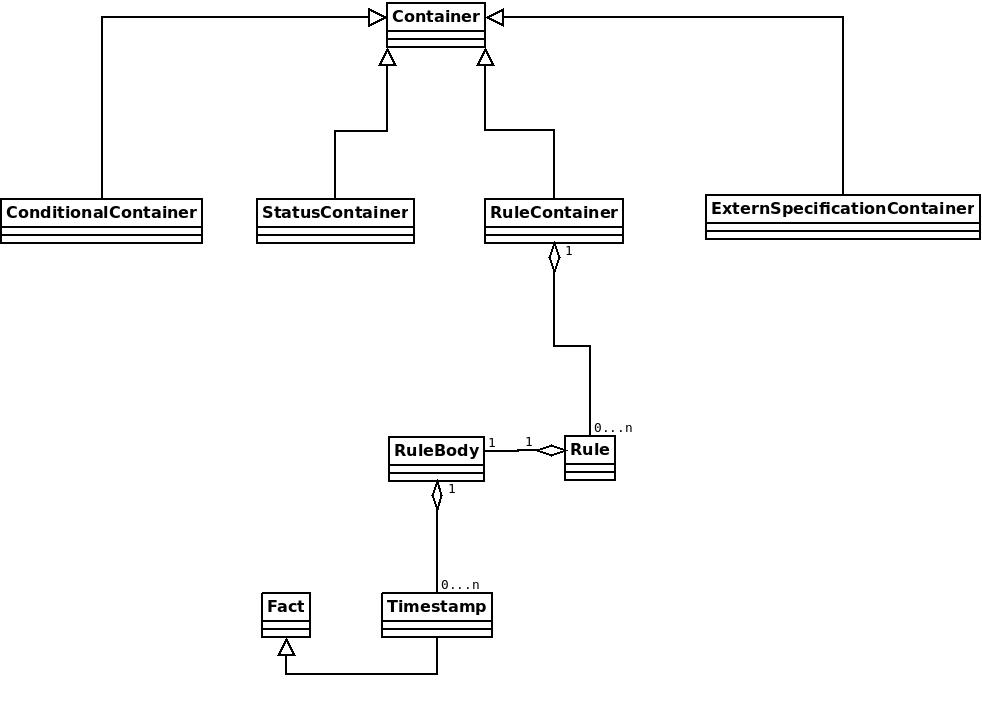
\includegraphics[width=0.9\textwidth]{Figures/Container}
	\caption{Interne Datenstruktur}
\color{red} TODO Grafik fertig machen, wenn Programm fertig
	\label{fig:container}
\end{figure}

\textbf{Transformation und Ergänzung der Regeln}\\
Nachfolgend wird ein Einblick gegeben, welche Transformationen und Ergänzungen der Listener vollzieht. Die Auflistung ist nicht vollständig, sondern skizziert nur die wichtigsten Ergänzungen.

Um dem Nutzer eine möglichst intuitive Definition der Regeln zu ermöglichen, wird in den Regeln direkt der Name der Aktivität verwendet. Da es jedoch theoretisch erlaubt ist, mehrere Aktivitäten mit dem selben Namen zu versehen, wird intern für jede Aktivität eine taskID generiert, über die zusammengehörige Informationen identifiziert werden. So müssen alle Klauseln, die einen Namen für die Aktivität tragen, in zwei Klauseln geteilt werden.\newline \texttt{'Mark' executed 'Auftrag annehmen'} wird somit zu\newline \texttt{user\_executed(taskID, 'Mark'), task\_name(taskID, 'Auftrag annehmen')}.

Die wichtigste Aufgabe des Listeners ist es, den Regeln entsprechende Klauseln hinzuzufügen, die sicherstellen, dass die Regeln im richtigen Kontext angewandt werden - Intra-Instance, Inter-Instance oder Inter-Process. Intra-Instance Regeln gelten für Aktivitäten in der selben Prozessinstanz. Inter-Instance Regeln betrachten auch Aktivitäten, die aus unterschiedlichen Prozessinstanzen gehören, jedoch aus dem selben Prozessschema. Inter-Process Regeln gelten für alle Aktivitäten, unabhängig davon, zu welchem Prozess sie gehören. Aus diesem Grund werden Intra-Instanz Regeln um Klauseln erweitert, die jeder Aktivität die selbe Prozessinstanz aufzwingen.

Zeitpunkte und Zeitspannen werden in ms nach 1970 übersetzt um arithmetische Operationen zu ermöglichen.

%
% ALGORITHMUS
%
\subsection{Algorithmus Compliance Checker}
\label{sec:compliancechecker}
In diesem Abschnitt wird betrachtet, wie der Compliance Checker die Logs auf die Einhaltung der definierten Regeln prüft. Der Checker selber besteht aus \textit{start.pl} und \textit{main.pl}. Die Datei \textit{start.pl} enthält die Routine zum Starten der Untersuchung. In \textit{main.pl} sind alle nötigen Funktionen, um implizite Beziehungen herzustellen und die einzelnen Routinen für die verschiedenen Regeltypen.

Bevor die eigentliche Untersuchung beginnt, werden zuerst noch einige implizierte Klauseln zu der Prolog-Datenbank hinzugefügt. Es werden alle \textit{collaborators} berechnet, die an {critical\_task\_pairs} gearbeitet haben, weitere Beziehungen aus dem Rollenmodell und Verwandschaften ermittelt.

Schließlich wird für jede Regel geprüft, ob es eine Klausel gibt, die sie bricht.\\
\color{red} TODO vernünftiger erklären
\color{black}

Im Anhang \ref{AppendixE} befindet sich der Pseudocode für die Analyseprozedur.

%
% ERGEBNISSE
%
\subsection{Darstellung der Ergebnisse}
\label{sec:results}
Sollte eine Aktivität im Log gefunden werden, die eine Regel bricht, wird der User/Rolle mit Task Namen und Beschreibung der Regel in \textit{results.txt} geschrieben.

\begin{verbatim}
Modelchecker startet...
Searching for illegal executions by user...

"blabla"
Illegal execution found: 
User Mark executed Task 10

Searching for illegal executions by role...
Searching for missed executions by user...
Searching for missed executions by role...
Searching for illegal executions...
Modelchecker finished...
\end{verbatim}
\begin{figure}[!h]
\small \color{red} TODO aktualisieren, wenn Programm fertig
\caption{Beispiel Output}
\label{fig:sampleoutput}
\end{figure}
